% \chapter{Theoretical Background}
\chapter{Methodology and Model Validation}
Explain any component Used, then Theory behind it, what kind of information that we extract.

It desig Antenna and Antenna-Lens with Ansys HFSS.

On this Thesis we try validation with 3 solver from 2 application. First, SIONNA-RT with Ray-tracing method solver, HFSS SBR+ with tray-tracing appriximation with S-Parameter, then HFSS Hybrid which combine FEM and SBR+ solver with S-Parameter. 

After that we simulate with same setup to validate Model. at this setup with 3x3 system with focus on variance angular domain.

\section{Antenna}
\subsection{Antenna Model}
Explain about Antenna That will be used, It should be FarField Model, Explain Formulation about this.

\subsection{Antenna Types}
Explain about Antenna Patch, and Dipole/wire because it was used. ont his design with Basic Antena Theory to design it.


\section{Antenna Lens Design}
Antenna Lens Design is built on the Metasurface Transmitarray Lens Design. Also basic Theory about it.

\subsection{Metasurface Unit-Cell Design}
<Tambahin Dasar Theory duls>

    \begin{figure}[htbp]
        \centering
        \begin{minipage}{0.3\textwidth}
            \centering
            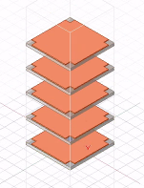
\includegraphics[width=\linewidth]{Images/Unitcell_Design.png}
            (a)
            % \label{fig:unitcell}
        \end{minipage}
        \begin{minipage}{0.48\textwidth}
            \centering
            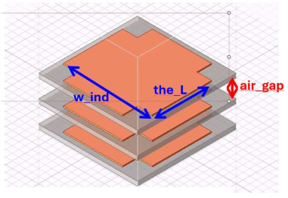
\includegraphics[width=\linewidth]{Images/Unitcell_Design_geometry.png}
            (b)
            % \label{fig:geometry}
        \end{minipage}
        \hfill        
        \caption{Unitcell design (a)5 layers with 1mm airgap (b)Sweep dimension}
        \label{fig:UnitcellDesign}
    \end{figure}
    The unit cell design is adopted from prior work on broadband metasurface superstrates, which enables polarization-independent wave focusing and gain enhancement at Ka-band frequencies.[1] As shown in Figure \ref{fig:UnitcellDesign}, the unit cell consists of a 5-layer stacked structure separated by air gaps, where the geometrical parameters such as patch width and layer spacing are varied to control the transmission response. 

    To evaluate the unit cell performance, a periodic simulation setup with Floquet ports is employed, as illustrated in Figure \ref{fig:UnitcellDesign}. This configuration allows the extraction of transmission characteristics under plane wave excitation.

    % \centering
\begin{figure}[htbp]
     \begin{minipage}{0.24\textwidth}
         \centering
         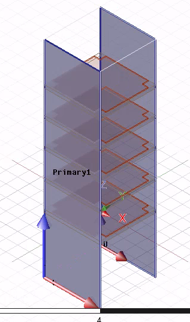
\includegraphics[width=\linewidth]{Images/FloqBoundary-1.png}
        %  \caption{Bloch Boundary 1}
        (a)
         \label{fig:floq_bound1}
     \end{minipage}
     \hfill
     \begin{minipage}{0.24\textwidth}
         \centering
         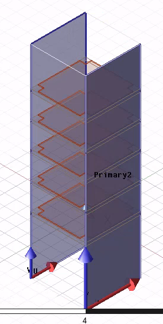
\includegraphics[width=\linewidth]{Images/FloqBoundary-2.png}
        %  \caption{Bloch Boundary 2}
        (b)
         \label{fig:floq_bound2}
     \end{minipage}
     \hfill
     \begin{minipage}{0.24\textwidth}
         \centering
         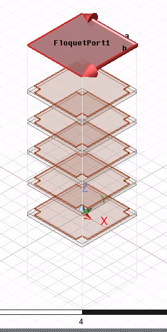
\includegraphics[width=\linewidth]{Images/FloqPort-1.png}
        %  \caption{Floquet Port 1}
         \label{fig:floq_port1}
         (c)
     \end{minipage}
     \hfill
     \begin{minipage}{0.24\textwidth}
         \centering
         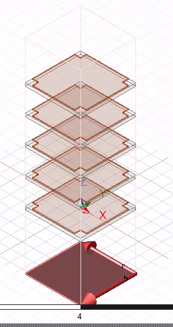
\includegraphics[width=\linewidth]{Images/FloqPort-2.png}
        %  \caption{Floquet Port 2}
         \label{fig:floq_port2}
         (d)
     \end{minipage}
     \caption{Simulation Setup Unit cell with FloquetPort}
     \label{fig:floquet_setup}
\end{figure}


    Using this simulation setup, the unit cell is optimized with respect to its transmission coefficient. As illustrated in Figure~\ref{fig:floquet_setup}, a range of geometrical variations is explored, and the final design is selected such that $S_{21}>-5\text{\,dB}$ at 38 GHz, thereby ensuring sufficient transmission efficiency for the lens application.

    This selection criterion follows directly from the power conservation principle\,[2]: the power incident on the unit cell must be fully accounted for by the reflected, transmitted, and dissipated components, as expressed in Equation~\ref{eq:power_conservation},
    \begin{equation}
        \left|S_{11}\right|^{2}+\left|S_{21}\right|^{2}+P_{loss}=1.
        \label{eq:power_conservation}
    \end{equation}
    From this relation, the transmitted and reflected power fractions can be expressed directly in terms of the simulated S-parameters as
    \begin{align}
        P_{T} &= \left|S_{21}\right|^{2} = 10^{\frac{S_{21,\text{dB}}}{10}}, \\
        P_{R} &= \left|S_{11}\right|^{2} = 10^{\frac{S_{11,\text{dB}}}{10}},
        \label{eq:power_definitions}
    \end{align}
    where the notation used above is summarized as follows:
    \begin{itemize}
        \item $S_{21}$: Transmission coefficient (forward transmission)
        \item $S_{11}$: Reflection coefficient (input reflection)
        \item $\left|S_{21}\right|^{2}$: Transmitted power ratio
        \item $\left|S_{11}\right|^{2}$: Reflected power ratio
        \item $S_{21,\text{dB}}$, $S_{11,\text{dB}}$: S-parameters in dB scale
        \item $P_{T}$: Transmitted power
        \item $P_{R}$: Reflected power
        \item $P_{\text{loss}}$: Power loss due to dielectric and conductor losses
    \end{itemize}
    Together, these relations justify the $S_{21}>-5\text{\,dB}$ criterion adopted above, as they guarantee that reflection and dissipative loss remain sufficiently small for the unit cell to operate efficiently as a transmitting element.

    \begin{figure}[htbp]
        \centering
        \begin{minipage}{\textwidth}
            \centering
            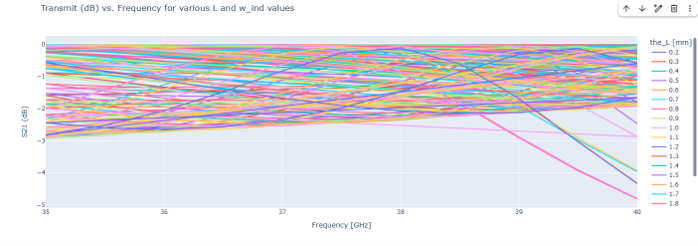
\includegraphics[width=\linewidth]{Images/UnitCell_Magnitude.png}
            % (a)
            
        \end{minipage}
        \hfill        
        \begin{minipage}{\textwidth}
            \centering
            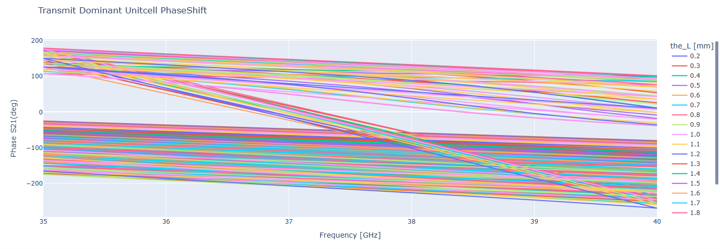
\includegraphics[width=\linewidth]{Images/UnitCell_Phase.png}
            % (b)
            % \caption{Transmission Phase}
            % \label{fig:UnitCell_Phase}
        \end{minipage}
        \caption{Transmit S21 in dB and phase shift angle deg.  with various dimension of unitcell}
            \label{fig:Unitcell_profile}
    \end{figure}

\subsection{Lens Phase Distribution / Cell Arrangement}
<Tambahkan Theory ddan gambar agar sesuai theoryn>

The working principle of the antenna lens is based on compensating the phase difference of a spherical wavefront.
When a point source is located at the focal point, the wave arriving at the lens aperture has different path lengths. To convert this into a planar wave, the lens must introduce a compensating phase [3], [4]:
    \begin{equation}
        \phi(x,y) = \frac{2\pi}{\lambda_{0}}\left(\sqrt{(x-x_{f})^{2}+(y-y_{f})^{2}+f^{2}} - f\right) + \phi_{\text{init}}
        \label{eq:phase_profile}
    \end{equation}

    \noindent where:
    \begin{itemize}
        \item $\phi(x,y)$: Required phase at position $(x,y)$
        \item $(x,y)$: Unit cell coordinates
        \item $(x_{f},y_{f})$: Center of the aperture
        \item $f$: Focal distance
        \item $\lambda_{0}$: Free-space wavelength
        \item $\phi_{\text{init}}$: Initial phase offset
    \end{itemize}
This equation ensures that all transmitted waves are in-phase, producing a collimated beam.
The metasurface antenna lens is designed with the following parameters:

\begin{table}[h!]
	\begin{center}
		\caption{Design parameters of the metasurface antenna lens}
		\label{table:lens_design_parameters}
		\begin{tabular}{|l|c|}
			\hline
			\textbf{Parameter} & \textbf{Value} \\
			\hline
			Antenna array size & $20 \times 20$ \\
			Antenna dimension & $44.24\,\text{mm} \times 44.24\,\text{mm}$ (@$2.367\,\text{mm} \times 2.367\,\text{mm}$ per unit cell) \\
			Number of layers & 5 \\
			Target focal point & 30\,mm \\
			Focal point after simulation & 14\,mm \\
			\hline
		\end{tabular}
	\end{center}
\end{table}

The required phase is implemented in a discrete manner across the aperture, where each unit cell represents a specific phase value.
As shown in Figure 4, the phase distribution forms a concentric (radial) pattern, indicating proper compensation of the spherical wavefront from the focal point. The symmetry also confirms that the phase is correctly centered. This phase distribution has been matched to the explored unit cell database to ensure practical realizability.
Furthermore, Figure 5 illustrates the physical realization of this phase distribution on the transmitarray structure, where each unit cell geometry corresponds to its assigned phase based on the explored unit cell responses.
Overall, the implemented phase profile closely follows the theoretical design, with minor deviations due to discretization.

% gambar Phase Distribution Phasenya
<Tambahkan Gambar Antenna Lens>

\subsection{Focal Characteristics}
To validate the designed transmitarray metasurface lens, a plane-wave incidence simulation is performed to assess its focusing performance under a realistic excitation scenario.

As illustrated in Figure~6, the metasurface is illuminated by a normally incident plane wave, with the propagation vector $\mathbf{k}$ oriented perpendicular to the lens aperture and the electric field $\mathbf{E}_{0}$ polarized orthogonal to $\mathbf{k}$, thereby ensuring uniform excitation across the entire unit-cell array.

<Gambar Setup Test Simulation>

The resulting transmitted field distribution is then examined to evaluate the focusing performance of the lens. As shown in Figure~7, the transmitted electric field is concentrated along the propagation axis and converges toward the target focal region, indicating that the incident plane wave is successfully focused by the metasurface.

Taken together, these results confirm that the phase distribution obtained from the explored unit-cell database is correctly realized by the transmitarray structure, yielding the intended focusing behavior and validating the overall lens design methodology.

<Gambar Hasil Simulation>

\subsection{Antenna Radiation Test}
<Tambahin Theory Transmitarray dengan Radiation Test>

To evaluate the far-field performance, a radiation test is conducted on the designed transmitarray to quantify its beam-focusing capability.

As shown in Figure~8, two aperture configurations, namely a $20 \times 20$ array and a $30 \times 30$ array, are considered in order to examine the influence of aperture size and focal distance on the radiation performance. In each configuration, the transmitarray is positioned in front of a source antenna so that its far-field radiation behavior can be characterized.

<Gambar Perbandingan Antenna dan dengan Antenna LEns>

The resulting three-dimensional radiation patterns are presented in Figure~9. It can be observed that incorporating the metasurface lens significantly enhances the antenna directivity, yielding a substantially more focused main beam compared with the case in which the lens is absent.

<Gamba perbandingan Radiation PAttern Antenna dalam 3d>

<Gamba perbandingan Radiation PAttern Antenna dalam 2d>

Furthermore, the radiation patterns at different frequencies are shown in Figure 10. The results indicate that the antenna with the lens achieves higher gain and narrower beamwidth, confirming the effectiveness of the designed phase distribution.

\section{MIMO Channel Modeling}

Place $N_R$ Receiver Antenna and $N_T$ Transmitter Antenna in free space. Receiver Antenna observe signal $y_i$ that construct by acumulated of many Transmitter signal $\mathbf{x}$ over medium between which called channel$\mathbf{H}$ including noise$\mathbf{n}$ . Then this system model can written as :
\begin{equation}
    \mathbf{y} = \mathbf{H}\mathbf{x} + \mathbf{n}
    \label{eq:basicMimo}
\end{equation}

this Basic system model can represent in many MIMO scheme including MIMO angular domain\cite{Tse2005}\cite{Challita2022}. In this thesis will try formulation on angular domain with scheme Receiver place on focal-plane behind antenna lens system ristic. Then we compare it conventional coplanar configuration.

\subsection{SVD/Singulat Value Decomposition}
    Explain about SVD
    
    Effective Rank, and condition Number

\subsection{Channel Quality Metrics}

\subsection{Channel Corellation Matrix}


\subsection{Channel Capacity}

\section{HFSS-Based Electromagnetic Simulation}
in this section We focused HFSS simulation. It was because, REsult of this simulation must be S-Paramater. Then We reformulated equation on \refeq{eq:basicMimo}.

\subsection{Simulation Setup}
Explain about Simulation Setup. we using 3x5x3 indoor Simulation that concrete Material around it.

\subsection{HFSS SBR+ Solver}
Result Simulation with SBR

ChannelEvaluation with this

\subsection{HFSS Hybrid Solver}
Result Simulation with Hybrid

ChannelEvaluation with this


\section{Cross-Validation Using Different Ray-Tracing Tools}
MIMO channel On SIONNA simulation using ray-tracing method. which using Common ray-tracing method. In this tools, MIMO Channel is construct with LoS Signal and also multipath that spread/spill from Transmitter Antenna to Receiver Antenna. 

Explain about channel extraction with \url{https://nvlabs.github.io/sionna/rt/em_primer.html}

\subsection{Simulation setup}
\subsection{Result Simulation}

* Comparison between HFSS and Sionna RT
* Comparison of propagation characteristics
* Channel matrix validation
* Comparison of channel correlation and capacity



* MIMO channel matrix formulation
Begin with Basic Communication Formulation y=Hx+n, Than from SISO, we MOVE to MIMO. Search from Book Fundamentals of Wireless Communication

* Channel correlation matrix
Theory for ot

* Singular value decomposition
Theory for ot

* Effective rank
Theory for ot

* Channel capacity
Theory for ot

\iffalse
% TODO: outline for remaining subsections
\begin{itemize}
    \item Geometry design (explain in figure)
    \item Substrate and conductor properties (explain in figure)
    \item Periodic boundary conditions (explain in figure)
    \item Floquet-port excitation (explain in figure)
    \item Geometrical parameter sweep [connector into Transmission Phase]
    \item Transmission Phase Characterization (explain 2 figures: magnitude graph, phase graph)
    \begin{itemize}
        \item Transmission magnitude $S_{11}$ and $S_{21}$ response
        \item Wrapped and unwrapped transmission phase
        \item Available phase range
        \item Unit-cell selection criteria
    \end{itemize}
    \item Lens phase distribution / cell arrangement
    \item Formulation for generating the unit cell
    \item Focal characteristics
    \begin{itemize}
        \item Show figure of the antenna lens focusing in the near field
        \item Show results for other incidence angles for verification (need at least 2,1)
    \end{itemize}
\end{itemize}
\fi
